\documentclass[oneside, a4paper, 12pt, brazil]{utfprcptex2}

\fontetipo{arial}

\instituicao{Universidade Tecnol�gica Federal do Paran�}
\unidade{C�mpus Corn�lio Proc�pio}
\diretoria{Diretoria de Gradua��o e Educa��o Profissional}
\coordenacao{Departamento de Computa��o}
\curso{Engenharia de Software}
\documento{Plano de Manuten��o de Software ISO/14764}
\area{Engenharia de Software}
\titulo{Gulosoo}
\autor{Josiel Faleiros, Rafael Santos}
\cita{SOBRENOME, Nome}
\local{Corn�lio Proc�pio}
\data{2018}

\begin{document}
	\capa
	\sumario
	\textual
	% Introduction
\chapter{Introdu��o} 

% Describe the system to be supported 
\section{sistema a ser suportado} 
O Gulosoo � um site que atualmente � um servi�o online para busca de estabelecimentos de consumo, e visualiza��o de informa��es importantes sobre estes estabelecimentos.

Os estabelecimentos podem ser buscados por cidade, onde o usu�rio pode selecionar a cidade que mora e ver todos os estabelecimentos desta cidade, organizados por aberto/fechado ou por localiza��o se o usu�rio tiver autorizado o acesso a sua localiza��o.

Quando um estabelecimento � selecionado, o usu�rio � redirecionado para a p�gina deste estabelecimento, onde pode encontrar informa��es importantes sobre o estabelecimento, como o seu card�pio mostrando produtos e seus pre�os, hor�rio de funcionamento, fotos do estabelecimento, promo��es atuais do estabelecimentos.
Possui integra��o com o sistema de mapas do Google (Google Maps) para mostrar o mapa de cada estabelecimento.

% Identify the initial status of the software
\section{status inicial do software} 
O site est� online atualmente, e pode ser acessado pelo endere�o: https://www.gulosoo.com.br


% Describe why support is needed 
\section{por que o suporte � necess�rio} 
O suporte � necess�rio, pois o site possui erros na interface que afetam a usabilidade do sistema.

% Identify the maintainer/support organization
\section{mantenedor/organiza��o do suporte} 
O grupo de suporte � composto pelos alunos Josiel Faleiros Alves e Rafael Nascimento Santos, alunos do curso de Engenharia de Software na UTFPR.

% Identify the specific software processes covered by the maintenance effort
\section{processos de software espec�ficos abrangidos pelo esfor�o de manuten��o} 
Cascata

% Describe any agreement protocols between customer and supplier 
\section{protocolos de acordo entre cliente e fornecedor}
Termo de aceite.

% a.7 Identify where maintenance will be performed
\section{onde a manuten��o ser� realizada}
A manuten��o ser� realizada na biblioteca da UTFPR C�mpus CP.

% a.8 Identify when maintenance will commence 
\section{quando a manuten��o come�ar�}
A manuten��o ocorrer� no per�odo: 04/18 -> 06/18

\pagebreak
% Identify costs to provide maintenance
\section{custos para fornecer manuten��o}
\begin{figure}[ht!]
	\caption{Diagrama de Caso de Uso}
	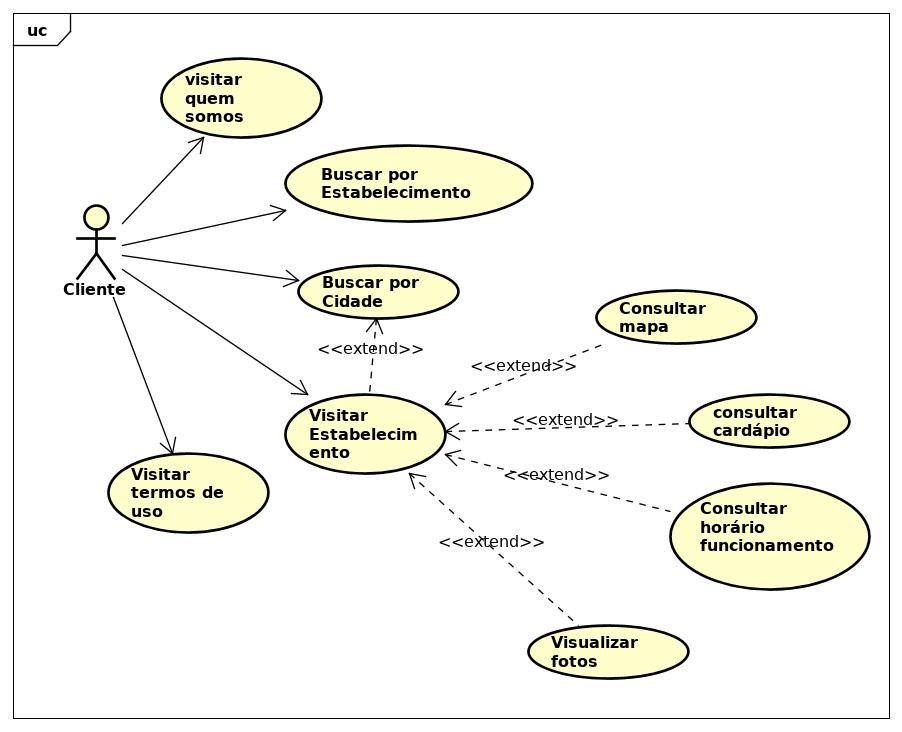
\includegraphics[width=\textwidth]{./a/casodeuso.jpg}
\end{figure}

\pagebreak
% Identify the schedule
\section{cronograma}
\begin{figure}[ht!]
	\caption{Cronograma}
	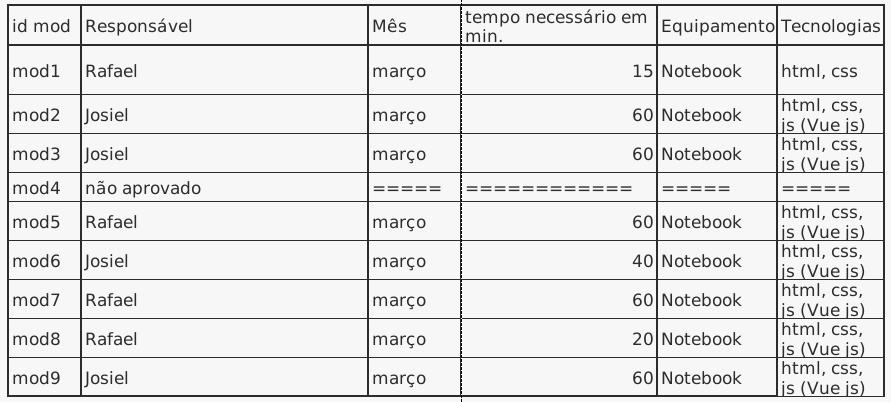
\includegraphics[width=\textwidth]{./a/cronograma.jpg}
\end{figure}
	% Identification and Control of the plan
\chapter{plano de controle}

% Identify the date of issue 
\section{data de envio}
8/4/2018

% Identify the status of the plan
\section{estado do plano}
Em andamento.

% Identify the issuing organization
\section{organiza��o emissora}
Gulosoo LTDA.

% Identify the approval authority
\section{autoridade de aprova��o}
Gerente de projeto: Josiel
Equipe de manuten��o: Rafael

% Describe the modification procedure for the plan
\section{procedimento de modifica��o do plano}
Manuten��es corretivas e evolutivas.

% Insert a modification history section
\section{se��o de hist�rico de modifica��es}
Git foi usado para versionamento do software e documento.

% Insert a glossary
\section{gloss�rio}
N�o utilizado.
	% References (to higher level policies, procedures, and documents and to lower level plans and procedures providing additional details
\chapter{Refer�ncias (para pol�ticas, procedimentos e documentos de n�vel superior e para planos de n�vel inferior e procedimentos que fornecem detalhes adicionais)}

% Identify the documents placing constraints on the maintenance effort
\section{documentos que colocam restri��es no esfor�o de manuten��o}
N�o utilizado.

% Identify documents referenced by the maintenance plan 
\section{documentos referenciados pelo plano de manuten��o}
N�o utilizado.

% Identify any supporting documents supplementing or implementing the maintenance plan 
\section{documentos comprovativos complementando ou implementando a manuten��o do plano}
N�o utilizado.
	% Definitions 
\chapter{Defini��es}

% Define or reference all terms required to understand the maintenance plan
\section{termos necess�rios para entender o plano de manuten��o}
N�o utilizado.

% Describe all abbreviations and notations used
\section{abreviaturas e anota��es}
	% Maintenance concept
\chapter{conceito de manuten��o}

% Describe the concept, including the level of support for the system (e.g., only implementing corrective maintenance)  
\section{conceito, incluindo o n�vel de suporte para o sistema (por exemplo, apenas implementando a manuten��o corretiva)}
Implementando manuten��es corretivas e de melhoria.

% Identify the support period 
\section{per�odo de suporte}
Mar�o de 2018 at� Junho de 2018
	% Organization and maintenance activities
\chapter{Atividades de organiza��o e manuten��o}

% Organization and maintenance activities
\section{Fun��es e responsabilidades da pr�-entrega do mantenedor}

% Process Implementation
\subsection{Implementa��o do Processo}
A implementa��o ser� realizada em um Sprint.

% Establish Infrastructure 
\subsection{Infraestrutura}
N�o se aplica.

% Establish Human Resource Process 
\subsection{Processo de Recursos Humanos}
Ser� realizada uma reuni�o de planejamento do Sprint.

% Establish the Software Maintenance Process
\subsection{Processo de Manuten��o do Software}
Manuten��o corretiva e evolutiva.

% Develop the maintainability plan
\subsection{Plano de Manutenibilidade}
Na reuni�o ser� definido o Sprint Backlog que ser� seguido durante o Sprint.

% Monitor development execution for maintainability
\subsection{Monitorar a execu��o do desenvolvimento para manuten��o}
O monitoramento ser� feito atrav�s dos commits do Git.

% Develop the transition plan
\subsection{Plano de Transi��o}
N�o se aplica.

% Participation by the maintainer in development activities  
\subsection{Participa��o do Mantenedor nas Atividades de Desenvolvimento}
Participar� de todas as atividades.

% Interface with other organizations
\subsection{Interface com outras organiza��es}
N�o se aplica.

% Post-Delivery roles and responsibilities of the maintainer 
\section{Fun��es e responsabilidades p�s-entrega do mantenedor}

% Process Implementation
\subsection{Implementa��o do processo}

% Problem and Modification Analysis
\subsection{An�lise de Problemas e Modifica��es}


% Modification Implementation
\subsection{Implementa��o de modifica��o}

% Maintenance Review/Acceptance
\subsection{Revis�o / Aceita��o de Manuten��o}

% Migration
\subsection{Migra��o}
N�o se aplica.

% Retirement 
\subsection{Aposentadoria}
N�o se aplica.

% Problem Resolution (includes Help Desk)
\subsection{Resolu��o de Problemas (inclui Help Desk)}

% Train personnel (maintainer and user), as applicable 
\subsection{Treinar pessoal (mantenedor e usu�rio), conforme aplic�vel}
O treino do mantenedor ser� feito atrav�s de programa��o em par.

% Improve the process 
\subsection{Melhorar o processo}
Ap�s o termino do processo ser� realizada uma reuni�o de retrospectiva.

% Factors that determine organizational maintenance priorities
\subsection{Fatores que determinam prioridades de manuten��o organizacional}

% The process for assigning a priority to a work package 
\subsection{O processo para atribuir prioridade a um pacote de trabalho }

% How resources are assigned to prioritized work packages
\subsection{Como os recursos s�o atribu�dos aos pacotes de trabalho priorizados}

% The schedule estimating method 
\subsection{O m�todo de estimativa de cronograma}

% Interface with other organizations
\subsection{Interface com outras organiza��es}
N�o se aplica.

% Role of the operator
\section{Papel do operador}

% Acceptance testing
\subsection{Teste de aceita��o}
Teste manual

% Interface with other organizations
\subsection{Interface com outras organiza��es}
N�o se aplica.
	% Resources 
\chapter{Recursos}

% Personnel 
\section{Pessoal}

% Size of staff for the project 
\subsection{Tamanho da equipe para o projeto }
Tamanho da equipe: 2 pessoas.

% Software 
\section{Software}


% Identify  software  needed  to  support  system  (includes  system  plus SEE/STE/tools requirements) 
\subsection{Identificar o software necess�rio para suportar o sistema}
O software necess�rio � um sistema operacional com navegador instalado, podendo ser Google Chrome acima da vers�o 59.0.3071, ou Firefox acima da vers�o 50.0

% Hardware 
\section{Hardware}
Requisitos do hardware.

% Identify hardware needed to support system (includes system plus SEE/STE requirements) 
\subsection{Identificar o hardware necess�rio para suportar o sistema}

% Facilities 
\section{Instala��es}

% Identify facilities requirements
\subsection{Identificar requisitos de instala��es}
Possuir internet.

% Special procedural requirements (e.g., security, access rights, and documentation control)
\section{Requisitos processuais especiais (por exemplo, seguran�a, direitos de acesso e documenta��o ao controle)}
N�o h�.

% Cost estimating 
\section{Estimativa de custo}

% Describe the cost estimating method 
\subsection{M�todo da estimativa de custo}
Pontos por caso de uso.

% Documentation 
\section{Documenta��o}

% Software Quality Plan
\subsection{Plano de qualidade do software}

% Project Management Plan 
\subsection{Plano de Gerenciamento de Projeto}

% Configuration Management Plan
\subsection{Plano de Gerenciamento de Configura��o}

% Measurement Plan
\subsection{Plano de Medi��o}

% Development documents
\subsection{Documentos de desenvolvimento}

% Maintenance manuals
\subsection{Manuais de manuten��o}

% Verification Plan
\subsection{Plano de Verifica��o}

% Validation Plan
\subsection{Plano de valida��o}

% Test Plan, Test Procedures, and Test Reports
\subsection{Plano de teste, procedimentos de teste e relat�rios de teste}

% Training Plan 
\subsection{Plano de Treinamento}
O treinamento ser� realizado atrav�s de programa��o em par.

% User?s Manual(s)
\subsection{Manual(s) do Usu�rio}
N�o se aplica.

% Data management
\section{Gerenciamento de dados}
Github.

% Identify repositories 
\subsection{Reposit�rios}

% Other resource requirements (if needed)
\section{Outros requisitos de recursos (se necess�rio)}
N�o se aplica.

	% Process (how the work will be performed)
\chapter{Processo (como o trabalho ser� realizado)}

% Maintainer?s process (give an overview of the process, do not spell out the entire process in the maintenance plan)
\section{Processo de manuten��o (d� uma vis�o geral do processo, n�o especifique a totalidade processo no plano de manuten��o)}
\begin{figure}[h!]
	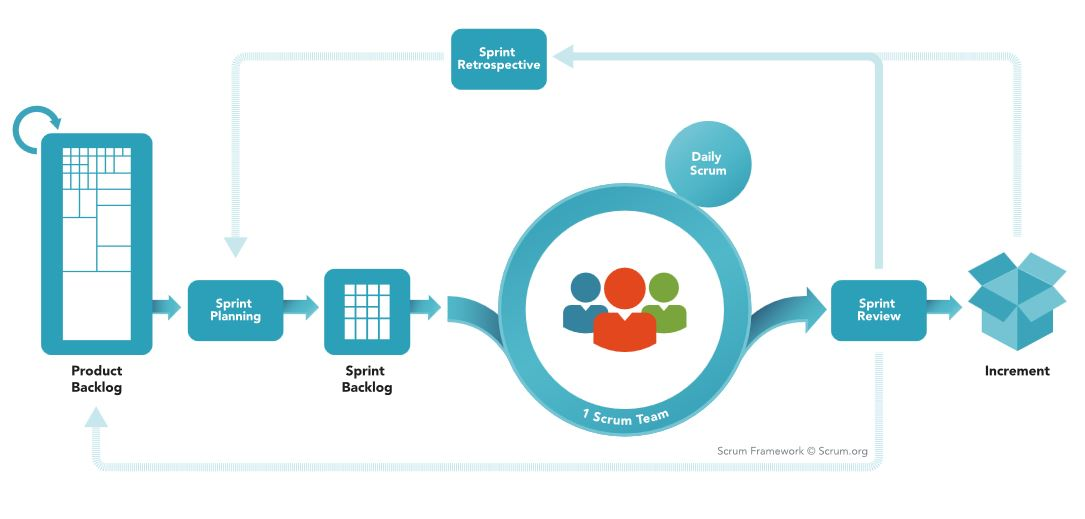
\includegraphics[width=\textwidth]{./h/scrum.jpg}
	\fonte{https://www.scrum.org/resources/what-is-scrum}
\end{figure}

% Defined process (identify actions to be performed for each activity in the process)
\section{Processo definido (identificar a��es a serem realizadas para cada atividade no processo)}
\begin{itemize}
	\item Backlog da manuten��o: Reuni�o para definir as modifica��es necess�rias.
	\item Sprint Backlog: Reuni�o de planejamento do Sprint.
	\item Implementa��o.
	\item Reuni�es di�rias do Scrum, que ser�o realizadas via Slack.
	\item Reuni�o de Review do Sprint para definir se a implementa��o ser� aceita.
	\item Reuni�o de Retrospectiva do Sprint para definir o que pode ser melhorado no processo.
\end{itemize}
	% Training 
\chapter{Treinamento}

% Identify training needs of the Maintainer and Users
\section{necessidades de treinamento do mantenedor e dos usu�rios}
O treinamento do mantenedor ser� feito atrav�s de programa��o em par, n�o h� necessidade de treinamento para o usu�rio.
	% Software maintenance control requirements 
\chapter{Requisitos de controle de manuten��o do software}

% Describe the deviation policy
\section{pol�tica de desvio}
N�o se aplica.

% Describe control procedures 
\section{procedimentos de controle}
Ser� feito atrav�s do quadro Kanban do Github.

% Identify quality control measures
\section{medidas de controle de qualidade}
Teste manual. As melhorias e corre��es implantadas.

% Describe standards, practices, and conventions
\section{padr�es, pr�ticas e conven��es}
N�o se aplica.

% Identify risks 
\section{riscos}
Risco de n�o terminar no prazo.
	% Maintenance records and reports
\chapter{registros e relat�rios de manuten��o}

% Describe how information will be collected and provided
\section{Descreva como as informa��es ser�o coletadas e fornecidas}

% Lists of requests for assistance, modification requests, or problem reports
\section{Listas de pedidos de assist�ncia, solicita��es de modifica��o ou relat�rios de problemas}

% Status of requests by categories 
\section{Status dos pedidos por categorias}

% Priorities of requests 
\section{Prioridades dos pedidos}

% Measurement data to be collected on maintenance activities
\section{Dados de medi��o a serem coletados em atividades de manuten��o}
	\postextual
	
\end{document} 